% -----------------------------------------------
% Vlastní text práce (kapitoly práce)
% -----------------------------------------------

% -----------------------------------------------
\chapter{Electronics for signal readout and analysis}
% -----------------------------------------------
The signals coming out the detector has to be properly preamplified, amplified and shaped. This  task requires special analog circuits with properly designed layout. 
In our case, we use instruments, modules and parts from two companies - ORTEC and CREMAT. When designing the spectrometric measurement chain, we select components in order to achieve sufficient parameters for our application - energy resolution, low dead time to increase maximum possible counting rates e.g. 
\par
The task of realizing the spectrometric chain can be fulfilled in two ways. The first and more straightforward way is to build it from stand-alone robust instruments and modules. This can be more practical approach for testing of the detectors themselves since we are not forced to solve problems arising from badly designed electronic circuits. However, these modules are usually very expensive, measurement setups build this way are unnecessarily large and have worse noise parameters than electronic circuits specially tailored for the given application.
\par
The second possibility is to design printed circuit board (PCB) with required functionalities from electronic parts, However it requires many electronic engineering skills and additional time for development. The analog PCBs are very hard to design. The pros are that the final product can be very compact, and the electronic parts and PCB manufacturing is much cheaper. In this thesis, we apply both methods for the development.



\section{PIN detector connection and support electronics}
\subsection{Voltage source}
The PN and PIN detectors require voltage bias to reduce the capacitance.
These voltage sources don't have to be stiff since the detector's current consumption is very low.
\par
Gas and scintillation detectors usually require high voltage source (hundreds or thousands of volts). These high voltages are usually supplied by switching power supplies.
However, these supplies are usually very noisy and since the semiconductors can be operated at much lower voltages, there is no need for them. The better alternative is charge pump build of capacitors and diodes, which requires lower frequencies to operate.
\subsection{Shielding and grounding}

In case of sensitive analog signal circuits, the electromagnetic shielding is a very important part. Sensitive circuits have to be surrounded by a metallic material from all sides, which is also correctly connected to GND (principle of the Faraday cage), otherwise the proper functionality can not be guaranteed. The electromagnetic field from an outside source usually induces currents in the shielding material, and thus the special care has to be taken to prevent these induced currents from flowing through the signal routes. The figure \ref{shielding} shows the difference between correct and wrong connection of shielding.

\begin{figure}[H]
 \centering
 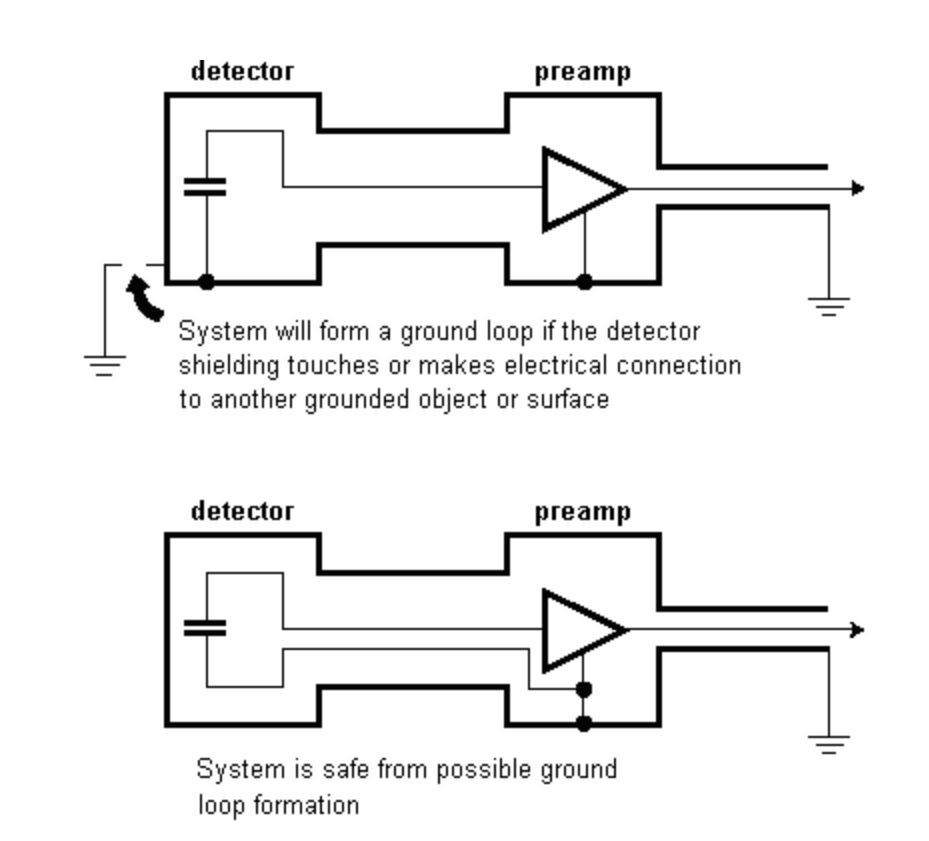
\includegraphics[scale=0.35, angle = 0]{./pictures/shielding.png}
 \caption{Schematic of wrong and correct connection of shielding \cite{appCSPnote}.}
 \label{shielding}
 
\end{figure}



\subsection{Cooling}
To reduce thermal noise and achieve better SNR it is necessary to cool the detector. The cooling can be achieved by various ways. In most setups, the appropriate solution can be provided by a peltier cooler. These setups with peltier are the easy to implement, however, their cooling efficiency is highly dependent on the ability to sink the heat from the hot side.

\section{Spectrometric chain}
The measurement chain for gamma spectroscopy is usually realized in following order - gamma detector, preamplifier, amplifier, multichannel analyser (MCA), microprocessor/computer.


\begin{figure}[H]
 \centering
 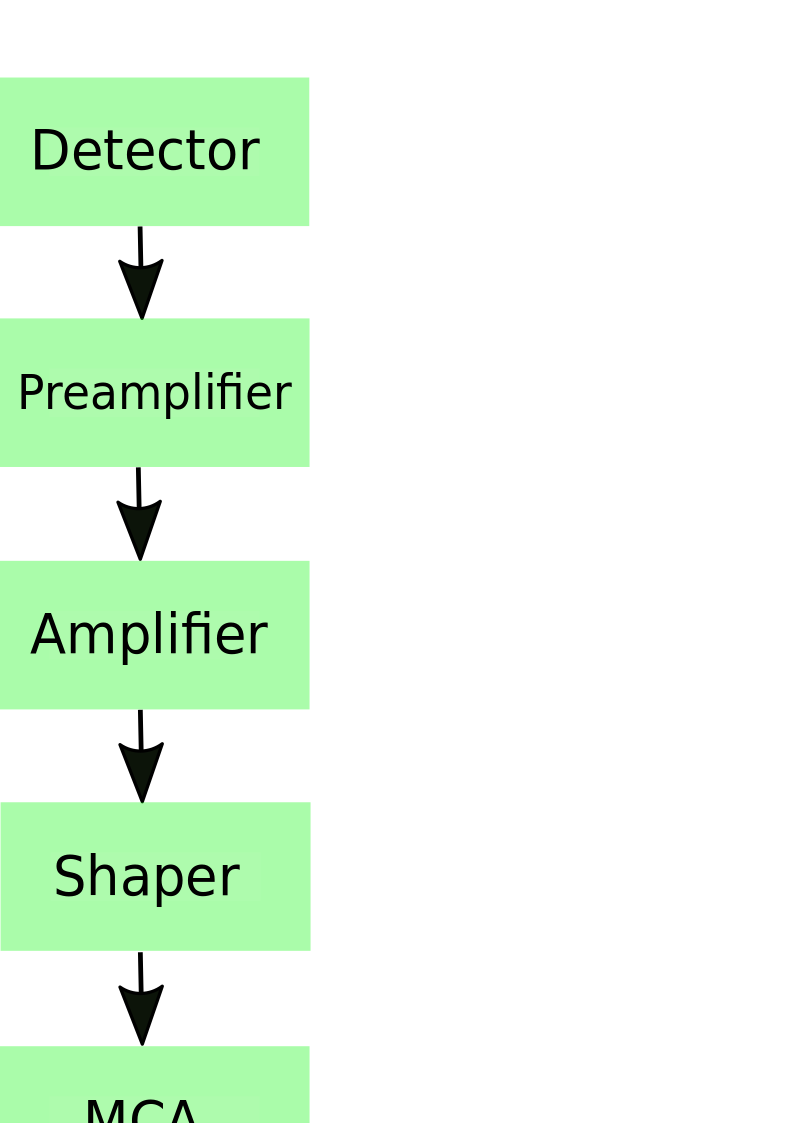
\includegraphics[scale=0.35, angle = 0]{./pictures/chain.png}
 \caption{Spectrometric chain.}
 \label{chain}
 
\end{figure}

\subsection{Pre-amplification}
The signal coming out of the PIN detector is weak, and it is also in form of charge (current pulse), so it is necessary to convert it into voltage pulse. For performing the charge-voltage conversion, one and the best solution is circuit called charge amplifier (also referred as a preamplifier). The principal functional scheme can be described by one opamp with a capacitor in feedback. The functionality is similar to $I/U$ transimpedance amplifier, but the charge amplifier works mainly as an integrator. In ideal case (opamp amplification $A >> 0$), the measured voltage per unit charge is approximately equal to:

\begin{equation}
\frac{dU}{dQ} = \frac{1}{C_{f}}.
\end{equation}


\begin{figure}[H]
 \centering
 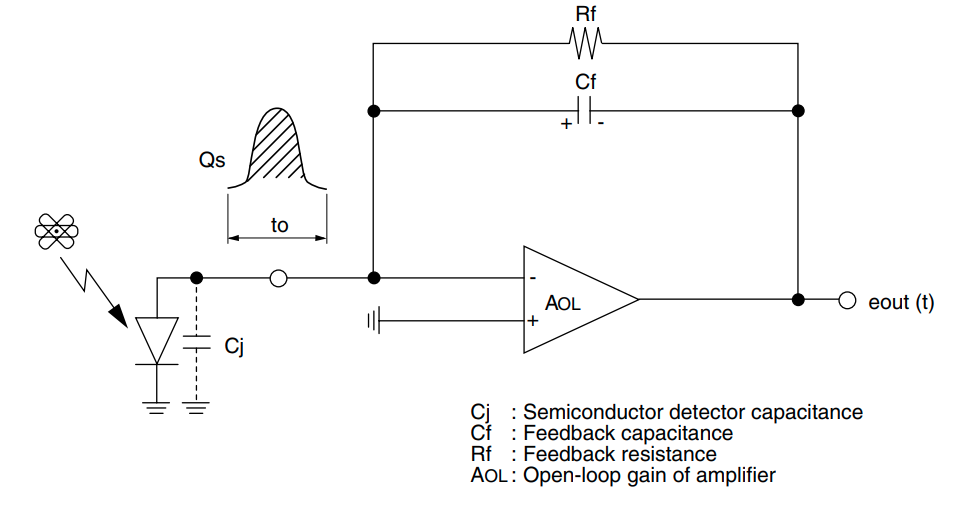
\includegraphics[scale=0.4, angle = 0]{./pictures/champlifier.png}
 \caption{Charge ampifier. $Qs$ is total charge of pulse and $to$ is the interval of charge generation inside the detector. Taken from \cite{charge}.}
 \label{trans}
 
\end{figure}



\par
In real circuit there is also a resistor parallel to the feedback capacitor. The feedback resistor slowly discharges the capacitor after a accumulation of charge, restoring the transimpedance amplifier to be ready to capture another pulse.

\begin{figure}[H]
 \centering
 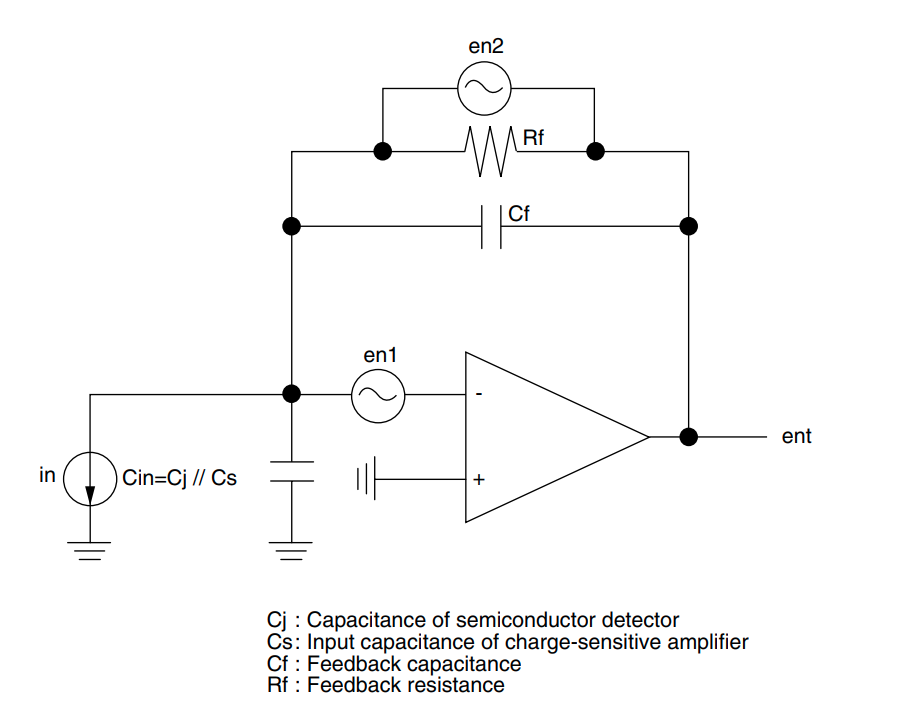
\includegraphics[scale=0.4, angle = 0]{./pictures/NoiseEquiv.png}
 \caption{Noise equivalent circuit for charge amplifier. Taken from \cite{charge}.}
 \label{trans}
 
\end{figure}


However, the functionality of charge amplifier is also negatively affected by an electronic noise, which depends on the values of the feedback resistance and capacitance and also on the internal parameters of the connected semiconductor detector and FET (field-effect transistor) inside the amplifier.

This electronic noise can be divided into three contributions, each described by euqations for noise voltages and currents \cite{charge}:

% on including the detector's capacitance $C_{\textrm{det}}$. Thermal noise dependency on $C_{\textrm{det}}$ of the first-stage FET transistor can be approximated by equation \cite{charge}:
\begin{itemize}

\item Thermal noise of first-stage FET:

\begin{equation}
en_1 = \sqrt{\frac{8}{3}\frac{kT}{gm}},
\end{equation}

where $k$ - Boltzmann constant, $T$ - absolute temperature and $gm$ - transconductance of FET. 

\item 

Shot noise caused by FET's gate current and detector's dark current:

\begin{equation}
in = \sqrt{2e(I_{\textrm{G}} + I_{\textrm{D}})},
\end{equation}

where $e$ - elementary charge, $I_{\textrm{G}}$ - gate leakage current of first-stage FET and $I_{\textrm{D}}$ - dark current of detector.



\item

Thermal noise caused by feedback resistance: 

\begin{equation}
en_2 = \sqrt{4KTR_{\textrm{f}}},
\end{equation}

where $R_{\textrm{f}}$ - the feedback resistance.

\end{itemize}


The square of total noise $ent^2(j \omega)$ is given by equation:


\begin{equation}
\begin{aligned}
ent^2(j \omega) = en_1^2 \cdot (1+\frac{C_{\textrm{in}}}{C_{\textrm{f}}})^2 + \{in^2 + (\frac{en_2}{R_{\textrm{f}}})^2 \}\frac{1}{(j \omega C_{\textrm{f}})^2},
\end{aligned}
\label{finalNoise}
\end{equation}

where the $C_{\textrm{f}}$ - the feedback capacitance and $C_{\textrm{in}}$ - the total input capacitance, resulting capacitance on the input of amplifier (there - parallel combination of detector's capacitance $C_{\textrm{j}}$ and amplifier's input capacitance $C_{\textrm{s}}$).   
\par
The first term in equation \ref{finalNoise} depends on the ration between the input capacitance $C_{\textrm{in}}$ and the feedback capacitance $C_{\textrm{f}}$ and thus the preamplifier's feedback capacitance has to be optimized in order to reduce the electronic noise.


\par
The charge sensitive preamplifiers modules usually also contain the second stage - common voltage amplifier. The internal scheme of CR-110-R2 charge amplifier made by Cremat Inc., which we use in the case of PCB design can be seen In the Fig. \ref{internal}.

\par

\begin{figure}[H]
 \centering
 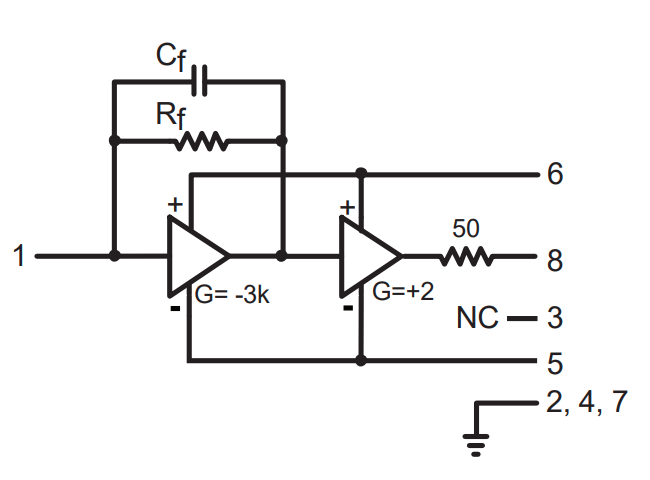
\includegraphics[scale=0.35, angle = 0]{./pictures/CRpreamp.png}
 \caption{Internal scheme of CR-110-R2 charge sensitive preamplifier \cite{cr110}.}
 \label{internal}
 
\end{figure}

The output voltage has the shape of exponential decay with amplitude defined by energy deposited into detector, short rise time (in orders of nanoseconds) and a longer decay constant (microseconds).


CR-110-R2 offers the conversion gain $G = 1.4$ V/pC, decay constant $\tau = 140$ $\mu$s CR-110-R2) and noise (FWHM) in silicon equal to 1.7 keV \cite{cr110}. It can be easily calculated, that for 14.4 keV photon, the output pulse has amplitude equal to $U_{A} = 0.8928$ mV. 
Note that the noise caused by the preamplifier is much larger than the intrinsic fano noise (FWHM = 185.4 eV).


\par
The modular version suitable for our application is ORTEC 142A charge preamplifier with $G = 1.016$ V/pC, $\tau = 500$ $\mu$s and noise in silicon equal to 1.6 keV \cite{ORTECpreamp}. Charge preamplifiers are usually very sensitive devices and can be very easily damaged by electrostatics. 

\par

Since the output of preamplifier is in order of millivolts, it has to be strongly amplified. Very fast and low noise amplifier consisting of multiple opamps is an appropriate solution of this problem.



\subsection{Shaping}

To perform the accurate energy discrimination, the pulse shape has to be altered from exponential decay shape by a shaping circuit. The shaping results into filtering the frequency band (reducing the noise) and also into shortening the long decay times of original exponential shapes. The shorter duration of pulses prevents the negative effect in which is one pulse superimposed onto another (pile-up effect).

\par
The Gaussian shape meets the sufficient parameters of SNR and duration \cite{Shapflify}. This type of shaping is usually achieved by several integration stages. The Cremat module CR-200-1us-R2.1 offers gaussian shaping with shaping time 1 $\mu$s \cite{cr200}. Its simplified internal schematic can be seen on fig.\ref{internal2}. 


\begin{figure}[H]
 \centering
 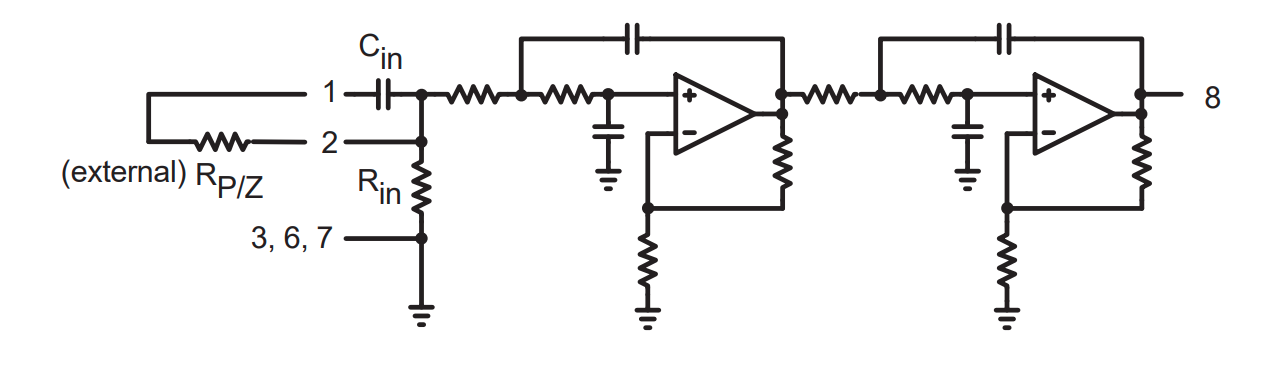
\includegraphics[scale=0.35, angle = 0]{./pictures/CRshaper.png}
 \caption{Internal scheme of CR-200 Gaussian shaping amplifier \cite{cr200}.}
 \label{internal2}
 
\end{figure}

However, shapers are usually very sensitive on the shape of the input pulse. They expect step-like input pulse. The deviation from the expected shapes may result into undefined shapes on output of the shaper. In modules the shapers are usually integrated along with amplifiers.

\subsection{Multichannel analysis (MCA)}
To obtain the full energy spectra information, it is necessary to measure and digitize pulse height of incoming pulses to perform energy discrimination and increment the corresponding channels. The multichannel analyser (MCA) can be employed for these purposes. The EASY-MCA-2K from ORTEC \cite{MCAOrtec}, which we use in experiments, is capable of processing Gaussian shaped pulses with shaping times from 0.25 $\mu$s to 30 $\mu$s and amplitudes ranging from 0 to +10 V.



% %%%%%%%%%%%%%%%%%%%%%%%% End of file %%%%%%%%%%%%%%%%%%%%%%%%